\documentclass[10pt]{beamer}
\usepackage[utf8]{inputenc}
\usepackage[T1]{fontenc}
\usepackage{lmodern}
\usepackage[spanish]{babel}
\usepackage{amsmath}
\usepackage{amsfonts}
\usepackage{amssymb}
\usepackage{graphicx}
%\usepackage[table]{xcolor}
\usetheme{Madrid}
\begin{document}
	\author{Daniel S. Parra}
	\title{Modelos PD - Toxicidad de Opioides}
	\subtitle{Morfina y Meperidina}
	%\logo{}
	%\institute{Fondo Nacional de Estupefacientes}
	%\date{}
	%\subject{}
	%\setbeamercovered{transparent}
	%\setbeamertemplate{navigation symbols}{}
	\begin{frame}[plain]
		\maketitle
	\end{frame}
	
	\begin{frame}
		\frametitle{Modelos PD Morfina}
		Se adaptaron los modelos de relación entre dosis y efectos adversos del siguiente artículo:\\
		\vspace{1.2cm}
		
		1. Galway JE, Morrison JD, Dundee JW. Dosage/Side-Effect Relationships of Morphine and Meperidine. Anesth Analg. 1973;52(4):536–41. \\
		
		\vspace{1.2cm}
		El análisis final fue realizado a partir de datos provenientes de 608 pacientes con morfina, y 872 pacientes con meperidina. 
	\end{frame}
	
	
	\begin{frame}
		\frametitle{Somnolencia vs Meperidina}
		
		\begin{table}[]
		\centering
		\small
		\begin{tabular}{|c|c|c|c|c|c|}
			\hline
			\multicolumn{6}{|l|}{\textbf{Modelo Logístico - Meperidina vs Somnolencia}}                    \\ \hline
			\multicolumn{6}{|l|}{\textbf{{Desviación de Residuos}}}                                        \\ \hline
			    Min      &    Q1    &  Mediana   &        Q3        &          Max          &              \\ \hline
			  -2.4536    & -0.9676  &   0.5529   &      0.8148      &        1.6636         &              \\ \hline
			\multicolumn{6}{|l|}{\textbf{Coeficientes}:}                                                   \\ \hline
			             & Estimado & Error Est. &     Valor Z      & Pr(\textgreater{}|z|) &              \\ \hline
			(Intercepto) & -1.6745  &   0.1997   &      -8.385      &   \textless{}2e-16    &     ***      \\ \hline
			   Dosis     &  1.4481  &   0.1248   &      11.606      &   \textless{}2e-16    &     ***      \\ \hline
			\multicolumn{6}{|l|}{Códigos Significativos:  0 ‘***’ 0.001 ‘**’ 0.01 ‘*’  0.05 ‘.’ 0.1 ‘ ’ 1} \\ \hline
			\multicolumn{6}{|l|}{(El parámetro de dispersión para la familia binomial se considera 1)}     \\ \hline
			\multicolumn{6}{|l|}{Desviación nula: 1143.06 en 871 grados de libertad}                       \\ \hline
			\multicolumn{6}{|l|}{Desviación residual: 973.51 en 870 grados de libertad}                    \\ \hline
			    AIC      & $\Delta$ &     gL     &        p         &          LL           &              \\ \hline
			   977.51    &  169.55  &     1      & \textless{}2e-16 &       -486.756        &              \\ \hline
			\multicolumn{6}{|l|}{Número de iteraciones de puntuación de Fisher: 4}                         \\ \hline
		\end{tabular}
		\end{table}
	\end{frame}
	
	
	\begin{frame}
		\frametitle{Somnolencia vs Morfina}
		
	\begin{table}[]
	\centering
	\small
	\begin{tabular}{|c|c|c|c|c|c|}
		\hline
		\multicolumn{6}{|l|}{\textbf{Modelo Logístico - Morfina vs Somnolencia}}                       \\ \hline
		\multicolumn{6}{|l|}{\textbf{{Desviación de Residuos}}}                                        \\ \hline
		    Min      &    Q1    &  Mediana   &    Q3    &          Max          &                      \\ \hline
		  -2.3971    & -1.0542  &   0.6251   &  0.8610  &        1.3058         &                      \\ \hline
		\multicolumn{6}{|l|}{\textbf{Coeficientes}:}                                                   \\ \hline
		             & Estimado & Error Est. & Valor Z  & Pr(\textgreater{}|z|) &                      \\ \hline
		(Intercepto) & -0.8461  &   0.2354   &  -3.595  &       0.000325        &         ***          \\ \hline
		   Dosis     &  7.3220  &   1.0284   &  7.120   &       1.08e-12        &         ***          \\ \hline
		\multicolumn{6}{|l|}{Códigos Significativos:  0 ‘***’ 0.001 ‘**’ 0.01 ‘*’  0.05 ‘.’ 0.1 ‘ ’ 1} \\ \hline
		\multicolumn{6}{|l|}{(El parámetro de dispersión para la familia binomial se considera 1)}     \\ \hline
		\multicolumn{6}{|l|}{Desviación nula: 748.81 en 607 grados de libertad}                        \\ \hline
		\multicolumn{6}{|l|}{Desviación residual: 684.19 en 606 grados de libertad}                    \\ \hline
		    AIC      & $\Delta$ &     gL     &    p     &          LL           &                      \\ \hline
		   688.19    &  64.623  &     1      & 9.07e-16 &       -342.094        &                      \\ \hline
		\multicolumn{6}{|l|}{Número de iteraciones de puntuación de Fisher: 4}                         \\ \hline
	\end{tabular}
\end{table}
	\end{frame}
	
	
	\begin{frame}
		\frametitle{Modelo PD - Somnolencia}
		\begin{figure}[H]
			\centering
			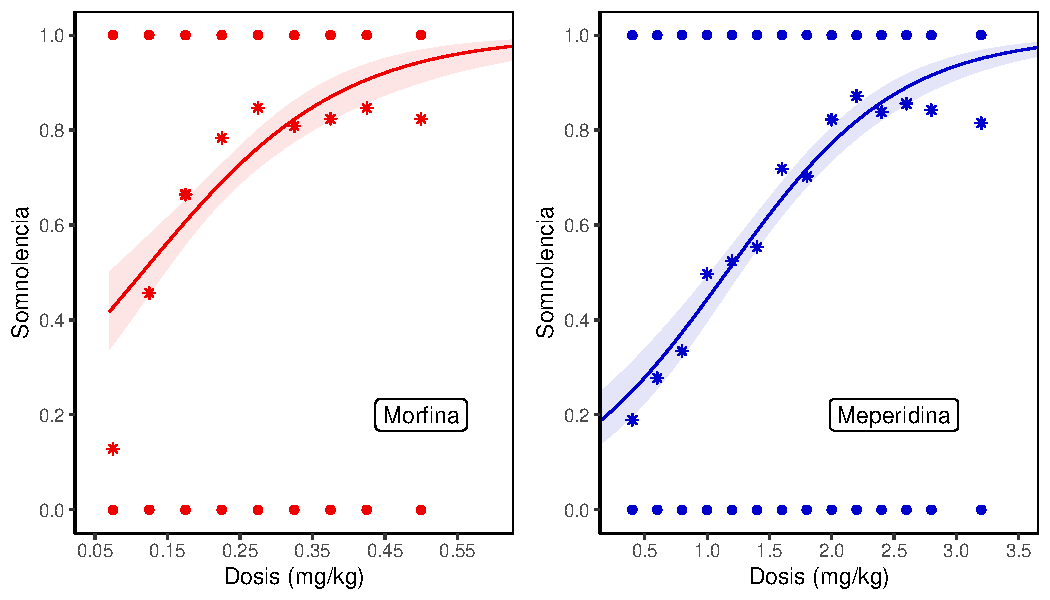
\includegraphics[width=0.9\linewidth]{Figuras/Somnolencia}
			\caption[Modelos Logísticos - Somnolencia]{Modelos Logísticos - Somnolencia}
			\label{fig:1}
		\end{figure}
	\end{frame}

















\begin{frame}
	\frametitle{Emesis vs Morfina}	
	\begin{table}[]
		\centering
		\small
		\begin{tabular}{|c|c|c|c|c|c|}
			\hline
			\multicolumn{6}{|l|}{\textbf{Modelo Logístico - Morfina vs Emesis}}                            \\ \hline
			\multicolumn{6}{|l|}{\textbf{{Desviación de Residuos}}}                                        \\ \hline
			    Min      &    Q1    &  Mediana   &    Q3    &          Max          &                      \\ \hline
			  -1.9203    & -1.3323  &   0.7366   &  0.9707  &        1.1976         &                      \\ \hline
			\multicolumn{6}{|l|}{\textbf{Coeficientes}:}                                                   \\ \hline
			             & Estimado & Error Est. & Valor Z  & Pr(\textgreater{}|z|) &                      \\ \hline
			(Intercepto) & -0.3508  &   0.2101   &  -1.670  &        0.0949         &          .           \\ \hline
			   Dosis     &  4.0444  &   0.8359   &  4.838   &       1.31e-06        &         ***          \\ \hline
			\multicolumn{6}{|l|}{Códigos Significativos:  0 ‘***’ 0.001 ‘**’ 0.01 ‘*’  0.05 ‘.’ 0.1 ‘ ’ 1} \\ \hline
			\multicolumn{6}{|l|}{(El parámetro de dispersión para la familia binomial se considera 1)}     \\ \hline
			\multicolumn{6}{|l|}{Desviación nula: 1208.7 en 871 grados de libertad}                        \\ \hline
			\multicolumn{6}{|l|}{Desviación residual: 1168.3 en 870 grados de libertad}                    \\ \hline
			    AIC      & $\Delta$ &     gL     &    p     &          LL           &                      \\ \hline
			   767.04    &  25.73   &     1      & 3.92e-07 &        -381.52        &                      \\ \hline
			\multicolumn{6}{|l|}{Número de iteraciones de puntuación de Fisher: 4}                         \\ \hline
		\end{tabular}
	\end{table}
\end{frame}

	\begin{frame}
	\frametitle{Emesis vs Meperidina}
	
	\begin{table}[]
		\centering
		\small
		\begin{tabular}{|c|c|c|c|c|c|}
			\hline
			\multicolumn{6}{|l|}{\textbf{Modelo Logístico - Meperidina vs Emesis}}                         \\ \hline
			\multicolumn{6}{|l|}{\textbf{{Desviación de Residuos}}}                                        \\ \hline
			    Min      &    Q1    &  Mediana   &    Q3    &          Max          &                      \\ \hline
			  -1.5931    & -1.1566  &  -0.8651   &  1.1460  &        1.5260         &                      \\ \hline
			\multicolumn{6}{|l|}{\textbf{Coeficientes}:}                                                   \\ \hline
			             & Estimado & Error Est. & Valor Z  & Pr(\textgreater{}|z|) &                      \\ \hline
			(Intercepto) & -1.03709 &  0.17755   &  -5.841  &       5.19e-09        &         ***          \\ \hline
			   Dosis     & 0.61749  &  0.09987   &  6.183   &       6.28e-10        &         ***          \\ \hline
			\multicolumn{6}{|l|}{Códigos Significativos:  0 ‘***’ 0.001 ‘**’ 0.01 ‘*’  0.05 ‘.’ 0.1 ‘ ’ 1} \\ \hline
			\multicolumn{6}{|l|}{(El parámetro de dispersión para la familia binomial se considera 1)}     \\ \hline
			\multicolumn{6}{|l|}{Desviación nula: 1208.7 en 871 grados de libertad}                        \\ \hline
			\multicolumn{6}{|l|}{Desviación residual: 1168.3 en 870 grados de libertad}                    \\ \hline
			    AIC      & $\Delta$ &     gL     &    p     &          LL           &                      \\ \hline
			   1172.3    &  40.37   &     1      & 2.10e-10 &        -584.16        &                      \\ \hline
			\multicolumn{6}{|l|}{Número de iteraciones de puntuación de Fisher: 4}                         \\ \hline
		\end{tabular}
	\end{table}
\end{frame}





	\begin{frame}
	\frametitle{Modelo PD - Emesis}
	\begin{figure}[H]
		\centering
		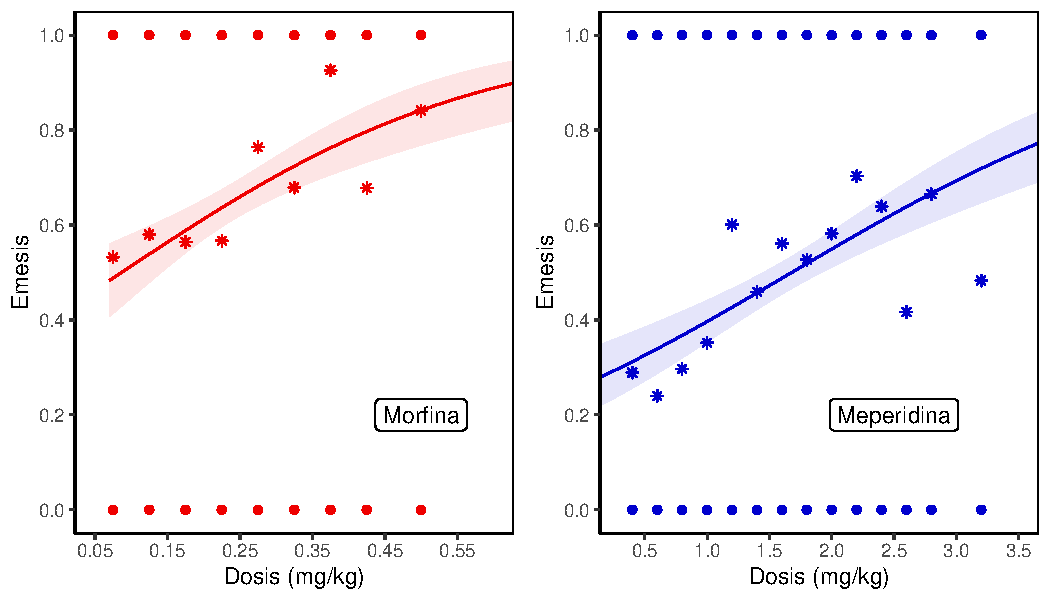
\includegraphics[width=0.9\linewidth]{Figuras/Emesis}
		\caption[Modelos Logísticos - Emesis]{Modelos Logísticos - Emesis}
		\label{fig:2}
	\end{figure}
	\end{frame}

	\begin{frame}
	\frametitle{Modelo PD - Aprehensión}
	\begin{figure}[H]
		\centering
		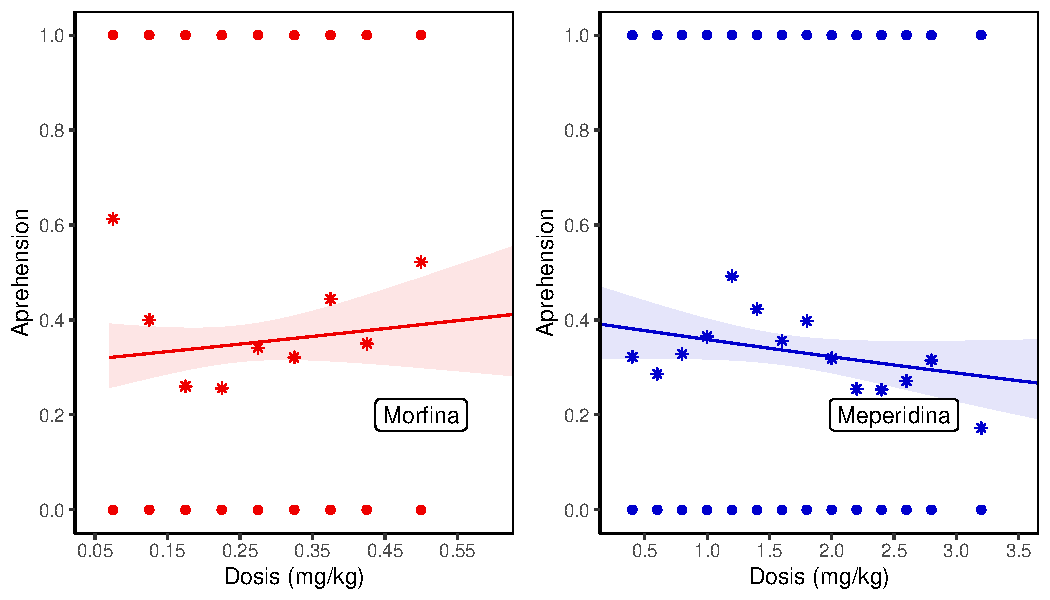
\includegraphics[width=0.9\linewidth]{Figuras/Aprehension}
		\caption[Modelos Logísticos - Aprehensión]{Modelos Logísticos - Aprehensión}
		\label{fig:3}
	\end{figure}
\end{frame}

\begin{frame}
	\frametitle{Modelo PD - Mareo}
	\begin{figure}[H]
		\centering
		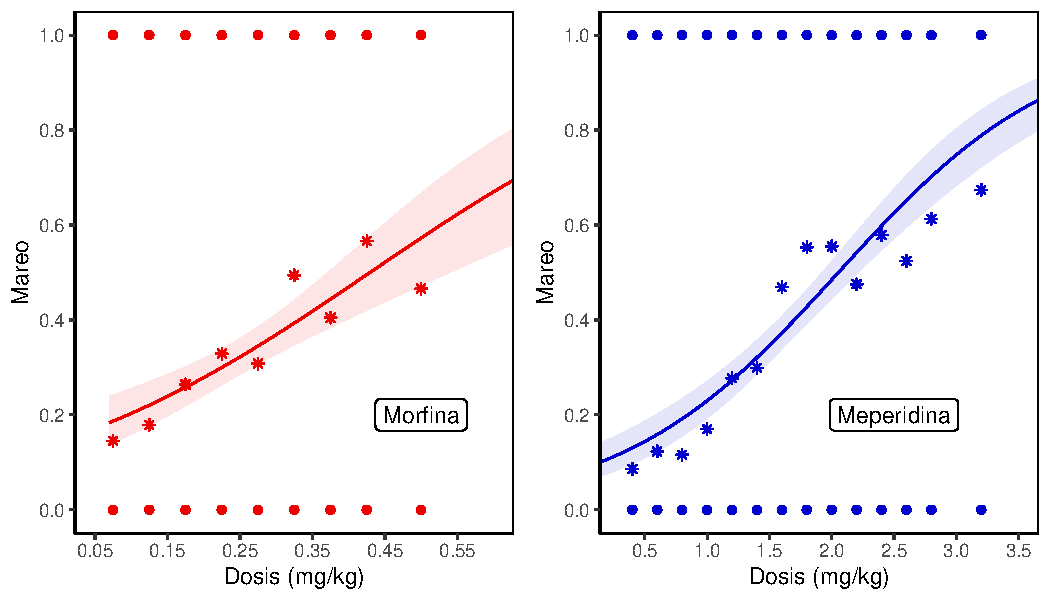
\includegraphics[width=0.9\linewidth]{Figuras/Mareo}
		\caption[Modelos Logísticos - Mareo]{Modelos Logísticos - Mareo}
		\label{fig:4}
	\end{figure}
\end{frame}



\end{document}